\section{Tower: from Functions to Architectures}
\label{sec:tower}

\begin{figure*}
  \begin{tabular}{p{0.36\textwidth}|p{0.30\textwidth}|p{0.33\textwidth}}
    \begin{smcode}
func :: Integer
     -> Def ('[Ref s (Stored IBool), Uint32]
             :-> ())
func period = proc "func" $ \textbackslash{}res currTime ->
  body $ do
    even <- assign (currTime .% (2 * p) <? p)
    store res even
    where
    p = fromIntegral period
    \end{smcode} &
    \begin{smcode}
blink :: ChannelSource (Stored IBool)
      -> Task ()
blink chan = do
  tx  <- withChannelEmitter chan
  res <- taskLocal
  onPeriod period $ \textbackslash{}now -> do
    call_ (func period) res now
    emit_ tx res
  where period = 100 :: Integer
    \end{smcode} &
% $
    \begin{smcode}
blinkApp :: Tower ()
blinkApp = do
  (tx,rx) <- channel
  task "blink" (blink tx)
  task "lightswitch" $
    onChannel rx $
      \textbackslash{}lit -> do
        ifte_ lit (turnOn light)
                  (turnOff light)
    \end{smcode}
  \end{tabular}
  \caption{Ivory (Column 1) and Tower (columns 2-3)}
  \label{fig:tower-ex}
\end{figure*}

In many embedded systems, programmers produce an entire system of software
that interacts with multiple input and output peripherals concurrently using a
real-time operating system (RTOS). Typical RTOSes provide just a few low-level
locking and signaling primitives for scheduling. Since microcontrollers do not
have virtual memory managment units (MMUs) found on larger processors, the RTOS
kernel can't protect the system against badly behaved user code. These
restrictions put significant burden on the programmer: she must ensure all tasks
and communication between tasks is implemented correctly.

Luckily, we already have Ivory in our toolbox, which guarantees memory-safety of
the generated code. During our initial development of SMACCMPilot, we found
ourselves writing high-quality C functions in Ivory.  But whenever we needed
``glue code'' to implement inter-process communication, initialize
data-structures, read the system clock, lock the processor, etc., we were forced
to abandon our well-typed world and tediously use C directly via Ivory's foreign
function interface.  Furthermore, the hand-written C is OS-specific, meaning it
would have to be rewritten for any OS port.

\paragraph{Extending Ivory}
The hand-written glue code was ruining both our productivity and our assurance
story. We wanted a different language to describe the structure the glue code
is required to implement, rather than using Ivory to write that code directly.
Our key insight was that such an EDSL could be built on ``top of'' Ivory, using
Ivory's code-generation facilities, without losing anything.

From these ideas, the Tower EDSL was born. You can think of Tower as an
extension to the Ivory language, designed to deal with the specific concerns of
multithreaded software architecture. Tower still allows the programmer to use
all the low-level power of Ivory for general programming, but uses a separate
language for describing tasks and the connections between them.  This is one of
the great productivity features of working with EDSLs: if you discover the
language you're using is difficult, tricky, or unsafe for solving a particular
problem, you can easily extend that language with a library, without modifying
the compiler.

In Tower, one specifies tasks and communication channels that generates correct
Ivory implementations, as well as architecture description artifacts. Tower
hides the dangerous low-level scheduling primitives to the user, and it keeps
type information for channels (i.e. the datatype of the channel message),
expressed as Ivory types, in the Haskell type system.

Tower allows the programmer to describe a static graph of channels and tasks.
This is a restriction of the capabilties of most operating systems, which may
create and destroy tasks or communication datastructures at run-time. However,
for the intended use case in high assurance systems, a static configuration of
channels and tasks makes it easier to reason about memory requirements, and
permits the system to be analyzed for schedulability.

\paragraph{Multiple Interpreters}

%% \begin{figure}
%%   \begin{center}
%% 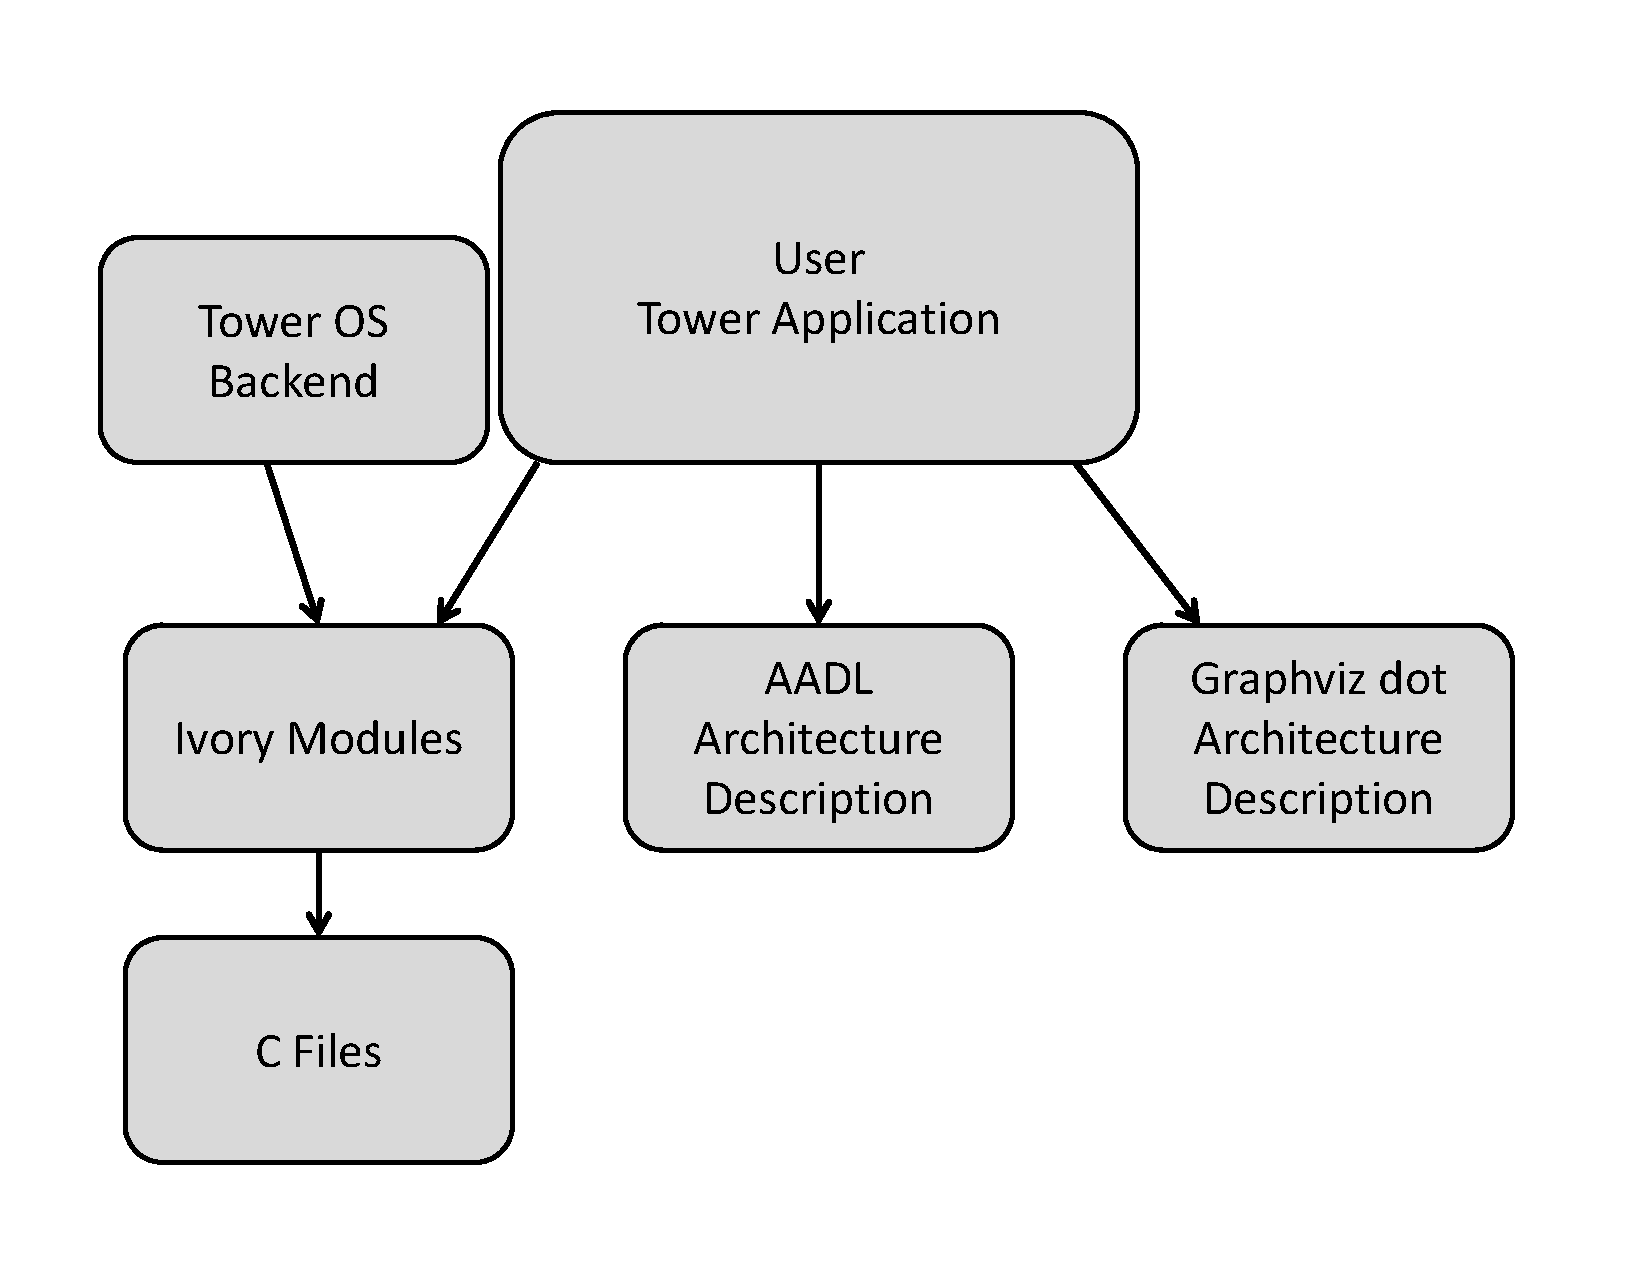
\includegraphics[width=6cm]{figures/tower-artifacts-dia}
%%   \end{center}
%%   \caption[Tower artifacts]{Tower artifact generation.}
%% \label{fig:towerArtifacts}
%% \end{figure}

In the Tower frontend, the programmer specifies a system that can be compiled into
multiple artifacts.

Tower is designed to support different operating systems via a swappable
backend. Since all code that touches operating system primitives is generated by
Tower, it is trivial for the user to specify a system and compile it for
different operating systems. Tower supports both the open-soure
FreeRTOS\cite{freertos} as well as the formally-verified
eChronos RTOS\cite{echronos} development by NICTA.

%% The static tower graph of channels and tasks also makes it possible to
%% describe the system architecture to external tools. 

Tower has a backend which generates a system description in the Architecture
Analysis and Design Language (AADL)~\cite{SAE:AADL}. We also built a backend for
the Graphviz dot language.  These output formats make it possible to visualize,
analyze, and automatically check properties about the system.  %% This is an
%% important feature when working with teams that may not all be literate in
%% Ivory/Tower.

We were pleased by the productivity improvements and correctness guarantees the
Tower language provided. In all, it took about 4 engineer-months to build Tower,
and a total of about 3000 lines of Haskell code.

\paragraph{Tower example}
In Figure~\ref{fig:tower-ex}, we sketch a small Tower example that is
representative of a device driver that blinks an LED at the rate of 100 ticks
(the duration of a tick is dependent on the RTOS backend to Tower used.)  Small
simplifications to Tower have been made in the code, eliding details relating to
code generation and backend selection.

Consider the first column of Figure~\ref{fig:tower-ex}.  The function takes an
integer and returns an Ivory procedure, which compiles to a C function.  The
procedure takes two arguments, a reference to a Boolean and a unsigned 32-bit
value.  The procedure creates a local variable binding within the language,
assigning to \cd{even} the value of an arithmetic expression.  The expression
takes a current time, which is a multiple of the period, and returns whether the
current time divided by the period is even or odd.  (Operators have a preceding
\cd{.} or a following \cd{?} for Boolean operators to avoid name-space collision
with Haskell operators.)  The result of the expression is stored into \cd{res}
reference.

The \cd{blink} task is defined in column two.  It takes a channel source and
returns a program in the \cd{Task} monad.  The task initializes first
initializes an emitter for the channel then creates a reference to private but
globally-allocated memory.  Every 100 ticks, an Ivory action is taken.  In this
case, the action is to make call an Ivory function, the one described in the
previous section, that toggles that value pointed to by \cd{res}.  This value
pointed to by \cd{res} is then emitted on the channel.

In the third column the program, defined in the \cd{Tower} monad, initializes a
channel between two tasks as well as the tasks themselves.  A channel, or queue,
consists of a transmit (\cd{tx}) and receive (\cd{rx}) endpoints, respectively.
The \cd{blink} task is an RTOS task that will send output to the
\cd{lightswitch} task, which toggles the LED based on the incoming Boolean
values.

%%  controls
%% the LED.  The \cd{lightswitch} task toggles the 

%% application \cd{} has three statements in the \cd{Tower} monad.
%% \cd{channel} gives a fresh \cd{Channel}. \cd{task "blink"} instantiates a task
%% defined by \cd{blink}, operating on the channel just created. \cd{task
%% "lightswitch"} defines another task with an event handler that takes the value
%% of the message recieved on the channel, and performs an action depending on
%% whether the boolean was true or false. Definitions for \cd{turnOn},
%% \cd{turnOff}, and \cd{light} are elided.


%% In the
%% example, we define a function \cd{blink} that takes a \cd{Channel (Stored
%%   IBool)} - that is, a Tower communication channel which contains messages of
%% booleans. The definition of \cd{blink} has two statements in the \cd{Task}
%% monad. \cd{withChannelEmitter chan} creates an \cd{Emitter (Stored IBool)} from
%% the \cd{Channel}, bringing that emmitter into scope for the particular task. The
%% second action, `onPeriod`, takes a period (in milliseconds) and an event handler
%% of type \cd{Uint32 -> Ivory eff ()}.

%% The definition of \cd{body}, the handler for the periodic event declared in
%% \cd{blink}, produces a fragment of Ivory code. The macro \cd{emit\_ tx} has type
%% \cd{IBool -> Ivory eff ()}. Its argument, \cd{even currTime}, calculates whether
%% the current time, modulo the period, is even or odd. We must make an \cd{Uint32}
%% - Ivory's 32-bit signed integer type - out of \cd{period :: Integer}, with
%% \cd{fromIntegral}.



